\documentclass[twoside,openright,a4paper,11pt,french] {report}

    % Packages
    % Règles de typographie françaises
    \usepackage[french]{babel}

    % Jeu de caractères UTF-8
    \usepackage[utf8]{inputenc}
    \usepackage[T1]{fontenc}

    % Inclure la bibliographie dans la table des matières comme une section
    \usepackage[numbib, nottoc] {tocbibind}	% numbib : section numérotée

    % Fonte élégante
    \usepackage{mathpazo}
    \usepackage[scaled] {helvet}
    \usepackage{courier}

    % pour certains symboles mathématiques peu fréquents, dont \square
    \usepackage{amssymb, amsfonts, amsmath, mathtools}

    % pour \EUR
    \usepackage{marvosym}

    % Utilisation de tableaux
    \usepackage{tabularx}
    
    % Utilisation d'url
    \usepackage[hidelinks]{hyperref}
    \urlstyle{sf}

    % Utilisation d'images
    \usepackage{graphicx}
    \setkeys{Gin} {keepaspectratio}	% par défaut : conserver les proportions

    % Utilisation de TikZ
    \usepackage{tikz}
    \usepackage{pgfplots}
    \pgfplotsset{compat=1.16}
    \usetikzlibrary{calc}

    % Utilisation des algorithmes
    \usepackage[linesnumbered,lined,boxed,commentsnumbered]{algorithm2e}

    % Définition des marges
    \usepackage[margin=25mm, foot=15mm] {geometry}

    % Utilisation de lipsum
    \usepackage{lipsum}

    % Utilisation des espaces
    \usepackage{setspace}


    % Définition des écarts

    % Écart entre les paragraphes
    \parskip=4mm
    \parindent=0mm

    % On enlève le saut de ligne quand on écrit des équations en inline
    \lineskiplimit=-\maxdimen%


    % On redéfini l'écart au dessus des paragraphes
    \renewcommand\paragraph[1]{\smallskip\noindent\textbf{#1}}

    % Le style de la page sera plain
    \pagestyle{plain}

    \raggedbottom

    \author{Nathanaël Derousseaux--Lebert}
    \title{Mémoire de stage}

\begin{document}

    % Page de garde
    \begin{titlepage}


    % Haut de la page
    \begin{minipage}{\linewidth}
        \begin{minipage}{0.25\linewidth}
            \centering
            
\includegraphics[width=\linewidth]{figs/logo-imt.png}
        \end{minipage}
        \hfill
        \begin{minipage}{0.5\linewidth}
            \centering
            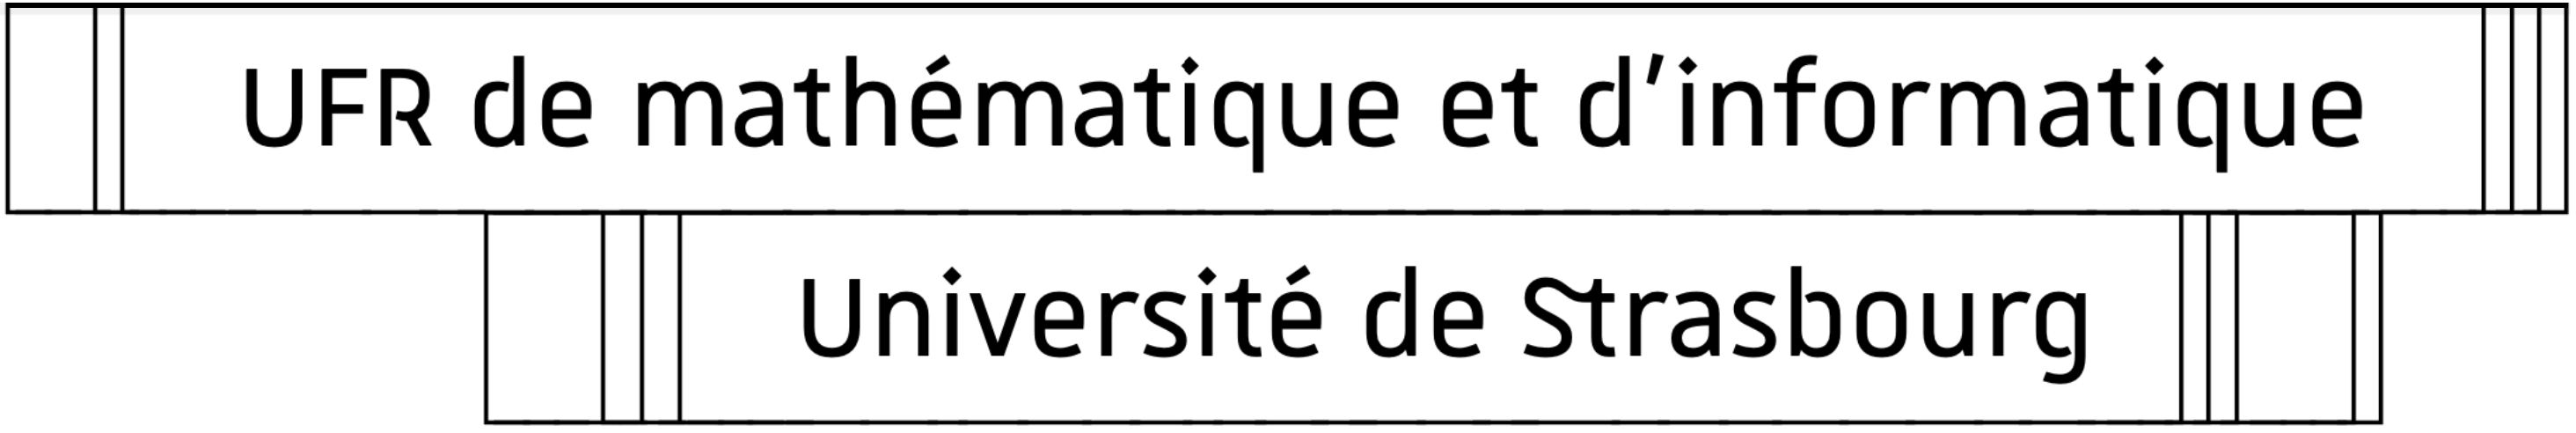
\includegraphics[width=\linewidth]{figs/logo-ufr.png}
        \end{minipage}
    \end{minipage}


    \vfill


    % Centre de la page
    \begin{center}
        {\Huge
            \textbf{
                {Adaptation de l'algorithme de}\\
                {compression de structures de données}\\
                {Blockchain MLS à un système à}\\
                {population variable}\\
            }
        }
        \vspace{0.4cm}
        {\LARGE
            Mémoire de stage\\
        }
        \vspace{0.1cm}
        {
            \Large
            Master Science et Ingénierie des Réseaux,\\ 
            de l'Internet et des Systèmes
        }
    \end{center}


    \vfill


    % Bas de la page
    \begin{center}
        {\Large
            \textbf{Nathanaël Derousseaux--Lebert}
        }\\
        Tuteur : LUDINARD Romaric\\
        Entreprise : IMT Atlantique\\
        Février 2024 - Août 2024\\

    \end{center}

\end{titlepage}

    \cleardoublepage%

    % Table des matières
    {
    \parskip=0pt
    \tableofcontents
}
    \cleardoublepage%

    % Introduction
    \chapter{Introduction}\label{chap:introduction}

	Dans le cadre de mon stage de fin d'études, j'ai travaillé au sein d'IMT
	Atlantique, une école de l'Institut Mines-Télécom, sur un projet de recherche
	visant à compresser les structures de données de type Blockchain. Le stage,
	d'une durée de 6 mois, a commencé le 5 février 2024 et se terminera le 2 août
	2024. Il s'est déroulé au sein du département d'enseignement et de recherche
	"Systèmes Réseaux, Cybersécurité et Droit du numérique" (SRCD) d'IMT
	Atlantique, situé à Rennes.

	Le projet de recherche sur lequel j'ai travaillé avait pour objectif de
	proposer une solution pour compresser les structures de données de type
	Blockchain, et ainsi faire face aux problématiques de scalabilité que ces
	structures posent. Une telle solution existait déjà, mais elle fonctionnait
	dans un cadre très particulier : le cas où la population du système reste
	constante. L'objectif était de généraliser cette solution pour qu'elle
	fonctionne dans un cadre plus large, utilisable dans le monde réel, où la
	population du système est susceptible varier. J'ai intégré une équipe de 3
	chercheurs qui travaillaient déjà sur ce projet depuis quelques mois. J'ai
	apporté ma contribution à la solution proposée.
	 
	Mon mémoire de stage se décompose en trois chapitres. Le premier est la mise
	en contexte avec une présentation de mon environnement de travail, et du
	projet plus global dans lequel s'est inscrit mon stage. Le deuxième chapitre
	est une revue de l'état de l'art sur les systèmes Blockchain et sur
	l'algorithme de compression que nous avons utilisé. Enfin, le troisième
	chapitre est une présentation de mon travail, des problématiques que j'ai
	rencontrées, et des solutions que j'ai apportées.

    % Contexte
    \chapter{Contexte}\label{chap:contexte}

    Mon stage de fin d'études s'est déroulé au sein d'IMT Atlantique, sur le
    campus de Rennes. Ce chapitre détaille le contexte global de mon stage en
    suivant un plan en entonnoir, allant de l'organisation générale d'IMT
    Atlantique jusqu'à mes missions spécifiques au sein du projet ANR
    \textit{Towards Public Blockchain for Self-Sovereign Identities}~\cite{anr},
    dans le cadre duquel mon stage s'est déroulé.

\section{IMT Atlantique}\label{sec:imt_atlantique} 

    % Imt atlantique
    IMT Atlantique, de l'Institut Mines-Télécom, est une école d'ingénieurs
    française issue de la fusion, en janvier 2017, de l'École nationale
    supérieure des mines de Nantes et de Télécom Bretagne. L'école possède trois
    campus situés à Brest, Nantes et Rennes. Elle propose des formations
    d'ingénieurs pluridisciplinaires couvrant les domaines des sciences, des
    technologies de l'information, de la communication, et des mathématiques. En
    termes de recherche, IMT Atlantique est structurée en douze départements
    d'enseignement et de recherche, regroupant des enseignants-chercheurs
    affiliés à différentes Unités Mixtes de Recherche (UMR) dont le GEPEA
    \footnote{\href{https://www.gepea.fr}{https://www.gepea.fr}}, l'IRISA
    \footnote{ \href{https://www.irisa.fr}{https://www.irisa.fr}}, et le
    Lab-STICC \footnote{\href{https://labsticc.fr}{https://labsticc.fr}}. Parmi
    ces douze départements, on trouve le département de Systèmes Réseaux,
    Cybersécurité et Droit du numérique (SRCD) sur le campus de Rennes, dans
    lequel j'ai effectué mon stage.

    % Le département SRCD
    Le département SRCD est composé à ce jour de 27 enseignants-chercheurs
    permanents, plus de 10 post-doctorants et ingénieurs contractuels, 31
    doctorants et 4 stagiaires. Les activités de recherche du département sont
    articulées autour de trois grands axes: les systèmes réseaux, la
    cybersécurité, et le droit du numérique. Les enseignants-chercheurs du
    département SRCD participent, avec des collègues d'autres institutions
    (\emph{e.g.,} Université de Rennes), à 6 équipes de l'IRISA, dont l'équipe
    SOTERN
    \footnote{\href{https://www.irisa.fr/sotern/}{https://www.irisa.fr/sotern/}}
    qui a accueilli mon stage.

    % Équipe SOTERN
    L'équipe SOTERN, pour Self-prOtecting The futurE inteRNet, s'articule autour
    du deuxième pilier de recherche du département SRCD~: la cybersécurité.
    C'est une équipe qui a été créée en début d'année 2023 et qui est dirigée
    par Guillaume Doyen, professeur à IMT Atlantique. L'équipe compte
    aujourd'hui 9 membres permanents, 1 post-doctorant, 6 doctorants et 5
    stagiaires. Les recherches de cette équipe se concentrent sur la conception,
    le développement et la validation de méthodes et d'outils pour
    l'auto-protection de l'Internet futur. Le projet ANR à l'origine de mon stage
    s'inscrit dans le cadre des recherches menées par l'équipe SOTERN.


\section{Projet BC4SSI}\label{sec:bc4ssi} 

    Mon tuteur, Romaric Ludinard, est le coordinateur du projet ANR intitulé
    BC4SSI~\cite{anr} (\textit{Towards Public Blockchain for Self-Sovereign
    Identities}). Ce projet s'inscrit dans l'axe E.3 /CES 25 de l'ANR, qui se
    concentre sur les verrous scientifiques relatifs aux réseaux de
    communication, architectures de réseau, et technologies logicielles, avec
    une attention particulière aux technologies Blockchain, et aux systèmes
    distribués. Plus spécifiquement, le projet BC4SSI à pour objectif de chercher
    des solutions aux verrous scientifiques et technologiques en lien avec les
    systèmes Blockchain, tels que décrit dans le rapport d'avril 2021 de la
    Direction Générale des Entreprises détaillant les principaux défis et enjeux
    de tels systèmes en France~\cite{dge}. Mon travail s'est concentré sur le
    verrou numéro 2, qui concerne la compression de structures de données de
    type Blockchain. J'ai rejoint le projet en février 2024, c'est-à-dire 12
    mois après le début de celui-ci. Quand je suis arrivé, un article de recherche
    était en cours de rédaction, et j'ai contribué à l'écriture des sections
    restantes.


\section{Mes missions}\label{sec:mes_missions}

    Les deux à trois premiers mois de mon stage au sein de l'équipe SOTERN ont
    été consacrés à la réalisation d'un état de l'art. Cette phase initiale
    était essentielle pour plusieurs raisons. La première était de me
    familiariser avec le sujet complexe de la Blockchain : cette période
    d'analyse des publications m'a aidé à identifier les solutions actuellement
    explorées dans le domaine. La seconde raison était de commencer à
    appréhender les outils et les concepts utilisés dans notre article. La fin
    de cette phase documentaire a donc été un mélange entre la lecture de la
    littérature et la reconstruction des preuves mathématiques détaillées dans
    les articles les plus proches de notre sujet, afin d'acquérir une
    compréhension fine des outils dont j'allais avoir besoin pour la seconde
    partie de mon stage.

    La seconde partie de mon stage a été consacrée à la rédaction de l'article
    de recherche. L'objectif était de proposer une solution pour compresser les
    structures de données de type Blockchain. Une telle solution existait déjà,
    mais elle fonctionnait dans un cadre très particulier : le cas où la
    population du système reste constante. Nous avons donc cherché à généraliser
    cette solution pour qu'elle fonctionne dans le cadre plus large d'un système
    à la population variable. J'ai donc participé à la fabrication de plusieurs
    modèles pour décrire notre problème et aux travaux mathématiques nécessaires
    pour démontrer la validité de nos propositions. J'ai également créé un
    programme de calcul qui implémente nos modèles afin d'obtenir des résultats
    numériques.


\section{Environnement de travail}\label{sec:contexte_de_travail}

    Au quotidien, j'ai travaillé avec les 4 personnes qui constituaient le pôle
    Blockchain de l'équipe SOTERN. Romaric Ludinard, mon tuteur, enseignant
    chercheur à IMT Atlantique, Loïc Miller, post-doctorant à IMT Atlantique
    également, Dorian Pacaud, Stagiaire qui a commencé 1 mois après moi, et
    Emmanuelle Anceaume, Directrice de Recherche au CNRS, membre de l'équipe
    PIRAT\textbackslash\textquotesingle);
    \footnote{\href{https://www.inria.fr/pirat}{https://www.inria.fr/pirat}} de
    l'IRISA.

    \vspace{0.4cm}
    \begin{figure}[ht]
        \centering
        \sbox0{\begin{tabular}{rl}
		\tikz{\node[fill=red!40, draw=black, inner sep=1ex]{};} & IMT Atlantique\\
		\tikz{\node[fill=green!40, draw=black, inner sep=1ex]{};} & SRCD\\
		\tikz{\node[fill=blue!40, draw=black, inner sep=1ex]{};} & SOTERN\\
		\tikz{\node[shape=circle, dotted, line width=2pt, draw=black, inner sep=0.5ex]{};} & BC4SSI
	\end{tabular}}

\begin{tikzpicture}[scale=1]
		\begin{scope}[shift={(3cm,-5cm)}, fill opacity=1]
				
				% Ellipses
				\draw[fill=red!40, draw=black] (0,0) circle (4);
				\draw[fill=green!40, draw=black] (0.5,0) circle (3.5);
				\draw[fill=blue!40, draw=black] (1,0) circle (3);
				\draw[draw=black, dotted, line width=2pt] (4,0) ellipse (5.5 and 2.3);
		
				% Noms
				\node at (1.5,1) (r) {\small \textbf{Romaric Ludinard}};
				\node at (1.5,0.5) (l) {\small \textbf{Loïc Miller}};
				\node at (1.5,0) (d) {\small\textbf{Dorian Pacaud}};
				\node at (1.5,-0.5) (n) {\small \textbf{Nathanaël Derousseaux}};
				\node at (6.7,0) (e) {\small \textbf{Emmanuelle Anceaume}};
				
				% Légende
				\node[below=1cm, draw, rounded corners] at (7.5,6) {\usebox0};
		\end{scope}

\end{tikzpicture}
        \caption{Organigramme de mon environnement de travail}
        \label{fig:organigramme}
    \end{figure}

    Pour garantir une bonne coordination, nous nous retrouvions deux fois par
    semaine pour discuter de nos avancées, des difficultés rencontrées, et
    travailler ensemble. Durant ma phase documentaire, ces réunions étaient
    surtout l'occasion pour moi d'obtenir des éclaircissements sur les articles
    que j'avais lus, et de me donner des pistes pour continuer mon travail.
    Ensuite, durant la phase de recherche, ces réunions ont permis d'avancer sur
    la rédaction de l'article, en réfléchissant ensemble à comment résoudre les
    problèmes que nous rencontrions. Le reste du temps, je travaillais en
    autonomie, partant des discussions de nos réunions pour avancer sur mes
    tâches.


    % État de l'art
    \chapter{État de l'art}\label{chap:etat_art}

	La première partie de mon travail a consisté à réaliser un état de l'art sur
	les systèmes Blockchain. Le plan de ce chapitre suivra la chronologie de mes
	recherches. J'ai commencé par approfondir mes connaissances sur le
	fonctionnement général des Blockchains~\cite{bitcoin}, avant de
	m'intéresser aux modèles utilisés pour décrire l'évolution de tels systèmes
	(\cite{static_backbone} et \cite{dynamic_backbone}). J'ai ensuite étudié un
	algorithme de compression dans un modèle dit \textit{statique}~\cite{mls}.
	Enfin, j'ai étudié le travail déjà effectué par l'équipe avant mon arrivée.
	L'objectif de ce travail étant d'adapter l'algorithme de compression à un
	modèle \textit{dynamique}, plus proche de la réalité.

	En plus de la lecture approfondie des articles auxquels je fais référence,
	j'ai refait de nombreuses preuves et calculs des travaux présentés dans les
	sections \ref{sec:dynamic} et \ref{sec:mls}. Cela m'a permis de me
	familiariser avec les outils et les concepts qui allaient m'être nécessaires
	pour la suite de mon travail de recherche.

    J'ai pris la liberté de renommer certaines variables et notations présentes
    dans les articles, afin d'homogénéiser les notations entre elles, et de
    rendre ma présentation plus claire. Une liste des notations relatives à
    chaque section est disponible en annexe~\ref{chap:notations}.
    

\section{Les systèmes Blockchain}\label{sec:blockchain}

    Ma première lecture a été évidemment le livre blanc de Satoshi
    Nakamoto~\cite{bitcoin}. Ce document est la première publication sur le
    sujet et reste une référence incontournable. La Blockchain y est décrite
    comme une solution de paiement décentralisée, sans tiers de confiance. La
    sécurité  du système y est assurée par un historique partagé de toutes les
    transactions. Il est ainsi auditable par tous les participants. La sécurité
    de l'historique est assurée par un mécanisme de preuve de travail (abrégée
    PoW pour Proof Of Work), qui garantit son intégrité.

    Quand un utilisateur (Bob) de la Blockchain veut effectuer un paiement
    auprès d'un autre utilisateur (Alice), il crée une transaction. Bob signe
    cette transaction avec sa clé privée, puis la diffuse sur le réseau. Les
    autres participants peuvent ainsi vérifier que Bob est bien en capacité de
    dépenser les fonds qu'il veut envoyer, et qu'il ne se dédit pas. Pour cela,
    ils vérifient la signature de Bob, et qu'il n'a pas déjà dépensé ces fonds.
     
    La transaction est ensuite ajoutée à l'historique des transactions. Pour
    savoir si Bob est en capacité d'utiliser son argent, on parcourt
    l'historique des transactions en partant de la création de la Blockchain. On
    cherche alors toutes les transactions qui lui sont destinées, mais qu'il n'a
    pas encore dépensées. On appelle ces transactions des UTXOs. Bob peut alors
    présenter ces UTXOs pour prouver qu'il est en capacité de dépenser ces
    fonds.

    D'une manière générale, une Blockchain est une structure de données. Au
    cours de mon travail, je n'ai pas eu besoin de m'intéresser aux données
    stockées, mais uniquement à la structure de la Blockchain. C'est pourquoi
    dans le reste de ce mémoire, je parlerai de données applicatives, sans
    préciser leur nature.


    \subsection{Structure de la chaîne}\label{subsec:fonctionnement}
    
    % Structure de la Blockchain
    Chaque changement d'état des données applicatives est stocké dans des blocs.
    Chaque nœud de la Blockchain stocke une copie de la chaîne de blocs. Quand
    un nœud reçoit un changement des données applicatives, il stocke ce
    changement dans un bloc à la fin de sa chaîne. Il diffuse ensuite ce bloc
    sur le réseau. Les autres nœuds vérifient la validité du bloc, puis
    l'ajoutent à leur chaîne. La chaîne la plus difficile à créer est considérée
    comme la chaîne de référence. Chaque nœud du système peut posséder une
    chaîne légèrement différente des autres. En effet le réseau subit un temps
    de propagation. Un bloc en fin de chaîne peut donc se faire invalider par
    une autre chaîne ayant demandé plus de travail. Cette chaîne n'aurait pas
    encore été reçue par notre nœud initial. Les derniers blocs d'une chaîne
    sont donc instables. Malgré cette instabilité des derniers blocs, chaque
    chaîne du réseau possède un préfixe commun immuable.

    % La structure d'un bloc
    Un bloc est une structure de données que l'on peut représenter par un tuple
    $(h, d)$, où $h$ est le header du bloc (ses méta-données) et $d$ constitue
    les données applicatives. Le header contient plusieurs informations
    importantes, le timestamp de création du bloc, le numéro de version du
    protocole, etc. Mais surtout, il contient le hash ($\mathfrak{h}$) du bloc
    précédent. Ainsi chaque bloc est lié au précédent, formant une chaîne de
    blocs. Un adversaire qui voudrait modifier un bloc, devrait recalculer tous
    les blocs suivants, puisque cela modifierait le hash du bloc modifié, qui
    modifierait celui du suivant, et ainsi de suite jusqu'à la fin de la chaîne.
    Pour s'assurer qu'un tel recalcul soit impossible, on va utiliser un
    mécanisme rendant la tâche de création d'un bloc difficile: la preuve de
    travail (PoW).

    \vspace{1cm}
    \begin{figure}[ht]
        \centering
        % Objet : fleche avec un texte au milieu 
% Paramètres : point de départ, taille, texte

\newcommand{\fleche}[3]{
	\draw[<-, >=stealth, thick] (#1) -- +(#2);
	\path (#1) -- +(#2) node[midway, above] {#3};
}


% Objet : sous-blocs: x, y, largeur, hauteur, titre
\newcommand{\sousbloc}[5]{
	\begin{scope}[shift={(#1,#2)}]
		\draw[fill=gray!40] (0,0) rectangle (#3,#4);
		\node[anchor=north west] at (0.05,#4-0.1) {\small #5};
	\end{scope}
}

% Objet : blocs
\newcommand{\bloc}[3]{
	\begin{scope}[shift={(#1,#2)}]
		\draw[rounded corners=0.2cm, fill=gray!20] (0,0) rectangle (6,4.7);
		
		% Titre en haut à gauche
		\node[anchor=north west] at (0.2,4.5) {\textbf{#3}};

		% Premiere ligne : hash du bloc précédent + nonce
		\sousbloc{0.3}{3}{3.4}{0.7}{Hash du préc. bloc}
		\sousbloc{4}{3}{1.7}{0.7}{Nonce}
		
		% Deuxième ligne : reste du header
		\sousbloc{0.3}{2}{5.4}{0.7}{Reste du header}

		% Troisième ligne : données applicatives
		\sousbloc{0.3}{0.3}{5.4}{1.4}{Données applicatives}

	\end{scope}
}


\begin{tikzpicture}[scale=1]
	\begin{scope}[shift={(3cm,-5cm)}, fill opacity=1]
		\bloc{0}{0}{Bloc n°43}
		\bloc{8}{0}{Bloc n°44}

		\fleche{6,3.35}{2.28, 0}{\small $\mathfrak{h}$}
		\fleche{-1.98,3.35}{2.28,0}{\small $\mathfrak{h}$}


		% Add more blocs as needed
	\end{scope}
\end{tikzpicture}
        \caption{Structure des blocs dans une Blockchain}
        \label{fig:blocs}
    \end{figure}


    \subsection{Preuve de travail}\label{subsec:pow}

    Pour rendre la création d'un bloc difficile, il existe plusieurs mécanismes.
    Le plus connu est la preuve de travail (PoW), mais il en existe d'autres,
    comme la preuve d'enjeu (PoS)~\cite{PoS}, ou la preuve de capacité
    (PoC)~\cite{PoC}. L'idée générale est de demander au créateur du bloc
    (appelé mineur) de résoudre un problème difficile. En revanche, la
    vérification de la solution doit être facile, pour que les autres
    participants puissent facilement vérifier la validité du bloc. Dans le cadre
    de mon stage, je me suis intéressé à la preuve de travail, qui est le
    mécanisme utilisé par Bitcoin.

    % Fonctionnement des preuves de travail
    La preuve de travail consiste à trouver à trouver un nonce (noté $c$), tel
    que :

    \begin{equation}
        \mathfrak{h}(c, h, d) < T
    \end{equation}

    Avec $\mathfrak{h}$ la fonction de hashage, $h$ le header du bloc (contenant
    le hash du bloc précédent), $d$ les données applicatives, et $T$ la target,
    définie par le protocole. Ainsi, il faudra tester tout les entiers $c$
    jusqu'à trouver un nonce qui vérifie cette équation. Plus $T$ sera petit,
    plus il sera difficile de trouver un tel $c$, inversement, plus $T$ sera
    grand, plus il sera facile de le trouver. On définit la difficulté comme
    l'inverse de la target $D = 1/T$.

    Afin de garantir que la création d'un bloc soit difficile, la difficulté est
    ajustée régulièrement. En effet, si le réseau au global augmente sa
    puissance de calcul, la difficulté de création d'un bloc risque de devenir
    trop faible et de permettre à un attaquant de créer des blocs plus vite que
    le reste du réseau. Pour éviter cela, la difficulté est ajustée par le
    protocole tous les 2016 blocs. Cet ajustement est paramétré de manière à ce
    que le temps moyen de création d'un bloc reste d'environ 10 minutes.

    % Les k derniers blocs de la chaîne sont instable
    Malgré ce mécanisme de preuve de travail, il est toujours possible que
    l'adversaire soit "chanceux" et trouve le nonce plus vite que les autres
    parties honnêtes du réseau. Cependant, statistiquement, il ne peut pas être
    "chanceux" à chaque fois. Le calcul de la probabilité de réussir à invalider
    un bloc à $k$ profondeur a été fait dans l'article de
    Nakamoto~\cite{bitcoin}, en modélisant le problème par un processus de
    Poisson :
    
    \begin{equation}
        1 - \sum_{i=0}^{k} \frac{\lambda^i e^{-\lambda}}{i!} (1-(q/p)^{k-i})
    \end{equation}

    Avec respectivement $q$ et $p$ les proportions de puissances de calcul de
    l'adversaire et de l'honnête (telle que $q + p = 1$) et $\lambda$ le taux de
    création de blocs ($\lambda = k(q/p)$). Ce calcul a permis d'estimer 
    qu'avec 1/3 de la puissance de calcul, l'adversaire a une probabilité de
    $P = 10^{-6}$ de réussir à invalider un bloc de profondeur 50.


\section{Le modèle statique}\label{sec:statique}

    Il existe un certain nombre de modèles pour décrire le fonctionnement des
    systèmes Blockchain. J'ai commencé par étudier un modèle
    statique~\cite{static_backbone} où la puissance de calcul de l'ensemble de
    nœud est fixée. Ce modèle est plus simple à étudier, mais reflétera moins la
    réalité qu'un modèle dynamique, où la puissance de calcul du réseau peut
    varier.
    

    \subsection{Présentation du modèle}\label{subsec:statique-presentation}

    Le modèle statique appréhende les systèmes Blockchain comme un ensemble de
    $n$ nœuds dont la puissance de calcul est fixée. Parmi ces $n$ nœuds, il y
    a $n-t$ nœuds honnêtes et $t$ nœuds malveillants. Les nœuds honnêtes suivent
    le protocole à la lettre, tandis que les malveillants peuvent tenter de le
    violer. Ce modèle se place dans une hypothèse synchrone, où le temps
    s'écoule en rondes. Par ailleurs, les canaux de communications sont
    considérés comme fiables, c'est à dire qu'il n'y a ni perte, ni altération
    ni duplication des messages émis. Ainsi, ces hypothèses assurent que tous
    les messages émis au cours d'une ronde sont reçus par leurs destinataires
    avant la fin de celle-ci. Qu'il soit malveillant ou honnête, chaque nœud ne
    peut faire qu'un nombre fixé $r$ requêtes par ronde à une fonction de
    hashage pour tenter de miner un bloc.

    \paragraph{Probabilité de réussite} On note $P_T$ la probabilité d'un unique
    nœud honnête de réussir à trouver un bloc en une seule requête à la fonction
    de hashage. On note $\kappa$ le nombre de bits de la sortie de la fonction
    de hashage. $T$ est la target utilisée pour la preuve de travail. Étant
    donnée que la fonction de hashage est indistinguable d'un processus
    uniforme, la probabilité de trouver un bloc en une seule requête est $P_T =
    T/2^\kappa$. On note $f$ la probabilité qu'au moins un nœud honnête trouve
    un bloc en une ronde. Cela revient à calculer l'espérance de la loi
    binomiale de paramètre $r$ et $P_T$, soit :

    \begin{equation}\label{eq:proba-bloc}
        f = 1 - (1 - P_T)^{r(n-t)}
    \end{equation}

    À partir de $f$, les auteurs introduisent trois variables aléatoires $X$,
    $Y$ et $Z$. $X_i = 1$ si au moins un nœud honnête trouve un bloc à la ronde
    $i$, $X_i = 0$ sinon. $Y_i = 1$ si exactement un nœud honnête trouve un bloc
    à la ronde $i$, $Y_i = 0$ sinon. $Z_i = 1$ si un nœud malveillant trouve un
    bloc à la ronde $i$, $Z_i = 0$ sinon. L'espérance et les variations de $X$,
    $Y$ et $Z$ sont facilement calculables puisqu'il s'agit de variables
    binomiales.

    \paragraph{Exécution typique} Le modèle introduit ensuite le concept
    d'exécution typique. Une exécution sera dite typique si les variables
    aléatoires $X$, $Y$ et $Z$ ne s'écartent pas trop de leur espérance, au plus
    d'un facteur $\varepsilon \in (0,1)$. Une exécution peut être dite typique
    uniquement si le nombre rondes considérées est suffisamment grand. On note ce
    paramètre $\Lambda \geq 2/f$. Pour finir, on partira du principe que la
    fonction de hashage est inviolable, c'est à dire qu'on omettra les cas de
    collisions. Les auteurs prouvent que la probabilité d'une exécution typique
    vaut $1 - e^{O(\varepsilon^2\Lambda f+\kappa-\log{L})}$, avec $L$ le nombre
    de rondes depuis le début du protocole.


    \subsection{Propriétés du modèle}\label{subsec:statique-proprietes}

    Avec ces outils, les auteurs du modèle ont pu prouver deux
    propriétés fondamentales du protocole Bitcoin si on reste dans le cadre
    d'une exécution typique. Ces deux propriétés sont le préfixe commun et la
    qualité de la chaîne. Le préfixe commun assure que les chaînes des nœuds
    honnêtes ont un préfixe commun important, tandis que la qualité de la chaîne
    assure que la proportion de blocs malveillants dans la chaîne des nœuds
    honnêtes est limitée.

    \paragraph{Préfixe commun} Le préfixe commun est garanti si la proportion de
    nœuds malveillants est inférieure à celle des nœuds honnêtes. Dans une
    exécution typique, si $t < n - t$, alors les chaînes des nœuds honnêtes ont
    un nombre de blocs $k$ à tronquer de la chaîne originale pour obtenir un
    préfixe commun qui est $k \geq 2\Lambda f$.

    \paragraph{Qualité de la chaîne} La qualité de la chaîne définit à quel
    point la chaîne des nœuds honnêtes est polluée par des blocs malveillants.
    La qualité de la chaîne sera idéale si la proportion de blocs appartenant
    aux malveillants est exactement égale à leur proportion de puissance de
    calcul. Les auteurs ont prouvé que dans une exécution typique, la qualité de
    la chaîne $t/n$ est garantie avec une probabilité écrasante si $t/n < 1/3$.

    
\section{Le modèle dynamique}\label{sec:dynamic}

    Dans un autre article~\cite{dynamic_backbone} les auteurs proposent une
    extension dynamique du modèle statique~\cite{static_backbone}. Ce modèle
    introduit la variation de la puissance de calcul du système au cours du
    temps. Il reprend les mêmes concepts que le modèle statique, mais rajoute un
    certain nombre d'outils mathématiques pour prendre en compte cette
    variation.


    \subsection{Présentation du modèle}\label{subsec:dynamic-presentation}

    La principale différence entre le modèle statique et le modèle dynamique est
    que le nombre de nœuds $n$ n'est plus fixé. Or, pour maintenir un rythme
    de création de blocs constant, le protocole doit ajuster la difficulté de
    création de blocs. Ainsi, si le nombre de nœuds augmente, la difficulté
    doit augmenter, inversement si le nombre de nœuds diminue. Donc la
    difficulté devient variable.

    \paragraph{Fonction de recalcul de la target} Pour ajuster la difficulté, le
    protocole doit recalculer la target $T$ tous les $J$ blocs ($J = 2016$ blocs
    dans le cas de Bitcoin). On nomme cet intervalle entre deux recalculs une
    \textit{epoch}. Les auteurs introduisent la fonction $D(\cdot)$ de recalcul
    de la difficulté. Cette fonction va être exécutée par chaque nœud à la fin
    de chaque epoch, pour définir la nouvelle target $T'$. La variation de la
    difficulté entre deux epochs est bornée par un facteur $\tau$ ($\tau = 4$
    dans le cas de Bitcoin). C'est à dire que $T/\tau \leq T' \leq T\cdot\tau$.
    Cela permet d'éviter des variations trop brutales de la difficulté, ce qu'un
    attaquant pourrait exploiter.

    \paragraph{Exécutions $(\eta, \theta)$-good} La fonction $D(\cdot)$ est
    exécutée par chaque nœud à la fin de chaque epoch. Sauf que chaque nœud ne
    dispose pas de la même information. En effet, le réseau subit un temps de
    propagation, et chaque nœud ne reçoit pas les mêmes blocs exactement au même
    moment. Il est donc légitime pour deux nœuds honnêtes de ne pas avoir
    exactement la même target $T$. Les auteurs introduisent donc le concept
    d'exécution $(\eta, \theta)$-good, qui assure que le taux de production des
    blocs honnêtes ne s'écartent pas trop du taux de production théorique
    attendu par le protocole. Une exécution sera dite $(\eta, \theta)$-good si :

    \begin{equation}
        \eta f \geq f(T, n) \geq \theta f
    \end{equation}

    Avec $f$ la nouvelle target calculée par le nœud, $T$ l'ancienne target,
    et $n$ le nombre de rondes considérées depuis la dernière epoch.

    \paragraph{Environnement $(\gamma, s)$-respecting} Un environnement sera 
    dit $(\gamma, s)$-respecting si la variation du nombre de nœuds est bornée
    d'un facteur $\gamma$ toutes les $s$ rondes. Cela assure que la variation
    du nombre de nœuds n'est pas trop brutale. En effet, il est raisonnable de
    supposer que dans la réalité, le nombre de nœuds ne varie pas trop vite.

    \paragraph{Variables aléatoires} Les auteurs modifient ensuite la définition
    des variables aléatoires $X$, $Y$ et $Z$ introduites dans le modèle
    statique. Avec une target dynamique, il ne suffit plus de considérer un bloc
    crée ou non, mais aussi de prendre en compte la target utilisée pour le
    créer. En effet, deux blocs créés avec des targets différentes n'ont pas la
    même probabilité d'être créés, ni la même importance lors de la comparaison
    entre deux chaînes. Les auteurs modifient donc les variables $X$, $Y$ et $Z$
    pour valoir $0$ si aucun bloc est créé, et $D$ si un bloc est créé avec une
    difficulté $D$.


    \subsection{Propriétés du modèle}\label{subsec:dynamic-resultats}

    À partir de ces nouveaux outils, les auteurs ont pu prouver deux autres
    propriétés importantes du protocole Bitcoin : la \textit{persistance} et la
    \textit{vivacité}. La \textit{persistance} assure qu'une donnée une fois
    inscrite dans la chaîne est immuable, tandis que la \textit{vivacité} assure
    qu'une donnée valide sera inscrite dans la chaîne.

    \paragraph{Persistance} La \textit{persistance} assure qu'une donnée une
    fois inscrite dans la chaîne est immuable. Dans une exécution typique, et un
    environnement $(\gamma, s)$-respecting, la \textit{persistance} est garantie
    quand la donnée est inscrite dans la chaîne à une profondeur $k$ telle que :

    \begin{equation}
        k \geq \frac{\theta \gamma J}{4\tau}
    \end{equation}

    \paragraph{Vivacité} La \textit{vivacité} assure qu'une donnée valide sera
    inscrite dans la chaîne. Les auteurs ont prouvé que dans une exécution
    typique, et un environnement $(\gamma, s)$-respecting, la \textit{vivacité}
    est garantie avec une probabilité écrasante en un temps fini.


\section{Algorithme de compression MLS}\label{sec:mls}
 
    Une Blockchain peut vite devenir très volumineuse. En effet, c'est une
    structure de données en ajout uniquement. Ainsi, aujourd'hui, la chaîne
    Bitcoin pèse plus de 450 Go après 15 ans d'existence. La chaîne Ethereum
    pèse quant à elle plus de 1 To après seulement 8 ans d'existence. De plus la
    croissance de telles chaînes est linéaire. Cela pose un problème d'accès à
    un tel réseau : si un nœud doit stocker l'intégralité de la chaîne, il lui
    faudra un espace de stockage important, et tous les appareils ne disposent
    pas d'un tel espace de stockage. C'est pourquoi il est important de trouver
    des solutions pour compresser la chaîne.
    
    Il existe aujourd'hui des solutions de compression et elles comportent
    toutes des compromis. J'ai étudié l'une d'entre elles, l'algorithme de
    compression \textit{Mining in Logarithmic Space} (MLS)~\cite{mls}. MLS est
    un algorithme de compression de la chaîne de bloc. L'article s'appuie sur
    les travaux du modèle statique~\cite{static_backbone}, c'est pourquoi il
    était important pour moi de travailler sur ce modèle avant de m'intéresser à
    MLS.
    

    \subsection{Présentation de l'algorithme}\label{subsec:mls_presentation}

    MLS fait partie de la famille des algorithmes NIPoPoWs (Non-Interactive
    Proofs of Proof of Work). Ces algorithmes permettent de prouver que les
    preuves de travail ont été effectuées sans avoir à effectivement posséder
    les blocs. L'algorithme MLS va échantillonner les blocs de la chaîne, et ne
    garder que les blocs les plus importants. Cependant, en échantillonnant les
    blocs, des données applicatives vont être perdues : on partira donc du
    principe que la chaîne que l'on va compresser effectue des snapshots de
    l'état applicatif à chaque bloc.
    
    Deux algorithmes seront nécessaires pour utiliser MLS : un algorithme de
    compression et un algorithme de comparaison, permettant de comparer deux
    compressés. Les deux algorithmes sont disponibles en annexe
    \ref{sec:mls_algo}.

    \paragraph{Niveau d'un bloc} Les auteurs introduisent le concept de niveau
    d'un bloc. Le niveau $\ell$ d'un bloc est défini comme le nombre de fois
    ou la target a été dépassée. Plus formellement :

    \begin{equation}
        \textrm{Le bloc } b \textrm{ est de niveau } \ell \Leftrightarrow
        \mathfrak{h}(b) \leq \frac{T}{2^\ell}
    \end{equation}

    Ainsi, un bloc de niveau $\ell$ est un bloc qui a dépassé la target de
    $2^\ell$ Étant donnée que la sortie de $\mathfrak{h}$ est uniforme, la
    probabilité qu'un bloc soit de niveau $\ell$ est $2^{-\ell}$. Donc tous les
    blocs seront de niveau 0, la moitié de niveau 1, le quart de niveau 2, etc.

    \paragraph{Algorithme de compression} L'algorithme MLS va échantillonner les
    blocs de la chaîne. Pour cela, il va d'abord chercher le niveau dit
    \textit{maximal} de la chaîne. Le niveau maximal est le niveau le plus haut
    qui possède au moins $2m$ bloc, $m$ étant un paramètre du système. On garde
    tous les blocs du niveau maximal. Ensuite, l'algorithme garde les $2m$
    derniers blocs de chaque niveau inférieur au niveau maximal, et les $m$
    derniers blocs du niveau supérieur.


    \paragraph{Chainage des blocs} Il est important de garder le bloc précédent
    dans la chaîne compressée pour pouvoir empêcher un adversaire de modifier un
    bloc au milieu de la chaîne. Cependant, comme l'algorithme ne garde pas tous
    les blocs, il est possible que le bloc précédent dans la chaîne initiale ne
    soit plus dans la chaîne compressée. Les auteurs propose de changer la
    structure de la Blockchain d'une liste simplement chaînée vers l'arrière à
    une liste à enjambement (\emph{skiplist}). Ainsi, chaque bloc contiendra le
    hash du dernier bloc de chaque niveau. On s'assure ainsi qu'on a toujours au
    moins une référence à un bloc qui sera contenu dans la chaîne compressée.

    \vspace{0.4cm}
    \begin{figure}[ht]
        \centering
        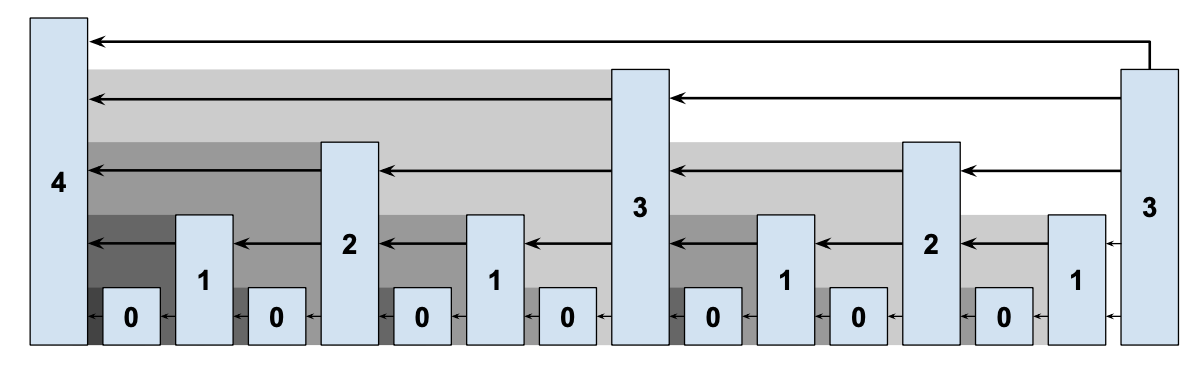
\includegraphics[width=0.8\textwidth]{figs/linking.png}
        \caption{Chainage des blocs dans MLS \cite{mls}}
        \label{fig:linking}
    \end{figure}

    
    \paragraph{Algorithme de comparaison} Les nœuds doivent être capables de
    comparer deux chaînes compressées pour choisir laquelle garder. L'algorithme
    de comparaison va chercher le dernier ancêtre commun de même niveau dans les
    deux compressés, et comparer les blocs à partir de ce point. Étant donné que
    l'algorithme de compression a gardé les blocs les plus \textit{rares}, le
    compressé ayant le plus de blocs de haut niveau sera celui qui témoigne
    d'une chaîne ayant demandé plus de travail avant la compression.


    \subsection{Propriétés de l'algorithme}\label{subsec:mls_proprietes}

    À l'aide des outils du modèle statique~\cite{static_backbone}, les auteurs
    ont pu prouver que l'algorithme MLS respecte trois propriétés importantes :
    la \textit{sécurité}, la \textit{concision} et l'\textit{idempotence}.
    
    \paragraph{Sécurité} La propriété de \textit{sécurité} assure que lors de la
    comparaison de deux chaînes compressées, l'algorithme de compression
    choisira le compressé honnête. Cette propriété a été prouvée dans le cas
    où l'adversaire possède moins d'un tiers du réseau, et que l'on est dans le
    cadre d'une exécution typique.

    \paragraph{Concision} La propriété de \textit{concision} assure que la
    taille de la chaîne compressée grandit de manière logarithmique par rapport
    à la chaîne originale $\mathcal{C}$ . Il a été prouvé que le compressé est
    de taille $2m \log{|\mathcal{C}|} + k$ avec $|\mathcal{C}|$ le nombre de
    blocs de la chaîne originale, $m$ le e paramètre de l'algorithme de
    compression, et $k$ les derniers blocs de la chaîne originale, que l'on ne
    compresse pas car ils sont instables.

    \paragraph{Idempotence} La propriété d'\textit{idempotence} assure que
    compresser une chaîne à laquelle on aurait préalablement ajouté un bloc est
    équivalent à compresser un compressé de cette chaîne à laquelle on aurait
    ajouté un bloc. Cette dernière propriété est importante pour garantir que
    l'on ne supprime pas des blocs dont on aurait besoin plus tard. La propriété
    d'\textit{idempotence} assure également que l'on puisse continuer de miner
    des blocs sur la chaîne compressée.
    

\section{MLS dans un modèle dynamique}\label{sec:mls_dynamic}


    L'algorithme de compression MLS~\cite{mls} a été conçu dans un modèle
    statique. Cependant, dans la réalité, le nombre de nœuds n'est pas fixé, et
    la difficulté de création de blocs doit être ajustée régulièrement. C'est
    pourquoi l'équipe de BC4SSI a travaillé sur une adaptation de l'algorithme
    de compression MLS à un modèle dynamique, plus proche de
    la réalité.

    La principale différence entre l'algorithme de compression MLS dans un
    modèle statique et un modèle dynamique est la variation de la difficulté.
    Cela a nécessité de modifier l'algorithme de compression et de comparaison
    pour prendre en compte cette variation (disponibles en annexe
    \ref{sec:mls_dyn_algo}). En effet, à présent, les difficultés des blocs sont
    prises en compte dans la comparaison des chaînes compressées.
    
    Les preuves ont aussi du être adaptées pour prendre en compte ce modèle
    dynamique. Ainsi, l'équipe a pu prouver qu'il était toujours impossible de
    supprimer un bloc de la chaîne compressée et que les propriétés de
    \textit{sécurité}, de \textit{concision} et d'\textit{idempotence} étaient
    toujours respectées dans la version dynamique de l'algorithme. Il a aussi
    été prouvé que la propriété du préfixe commun était toujours respectée en
    considérant les blocs du même niveau. C'est à dire que deux chaînes
    partagent un préfixe commun important de blocs de même niveau.

    \paragraph{Valeur de $m$} La valeur de $m$ est un paramètre important de
    l'algorithme de compression MLS. Il définit le nombre de blocs de chaque
    niveau que l'on garde dans la chaîne compressée. Choisi trop petit,
    l'adversaire risque de pouvoir créer une chaîne compressée plus difficile
    que la chaîne honnête par "chance". Choisi trop grand, la chaîne compressée
    deviendra trop volumineuse. Les auteurs de l'algorithme du modèle statique
    n'ont pas exprimé de valeur de $m$. Il s'agit pourtant d'un paramètre
    important pour utiliser l'algorithme dans la réalité. C'est pourquoi
    l'objectif de notre article est de proposer une valeur de $m$ pour
    l'algorithme de compression MLS dans un modèle dynamique. Ça sera l'objet de
    la suite de mon travail de recherche.


    % Réalisation
    \chapter{Réalisations}\label{chap:realisations}

	Dans ce chapitre, je détaille la seconde partie de mon travail de recherche :
	mes réalisations. En effet, ma mission était d'aider à finir l'article en
	cours d'écriture, dont j'ai présenté l'existant dans la section
	\ref{sec:mls_dynamic}. Ce chapitre présentera donc les travaux que j'ai
	réalisés pour aider à la finition de cet article.

	La première de mes réalisations a été de calculer la probabilité de créer un
	bloc pour un adversaire, sachant que celui-ci peut tricher sur la target $T$
	qu'il choisit. On a ensuite cherché à déterminer une valeur de $m$ qui
	permettrait de garantir les propriétés souhaitées pour l'algorithme MLS. Pour
	cela, on a exploré deux méthodes : une méthode par marche aléatoire, et une
	méthode par la ruine du joueur. La méthode par marche aléatoire n'a rien
	donné, le problème n'étant pas résolu à l'heure actuelle par la communauté
	scientifique. En revanche, la méthode par la ruine du joueur a fourni des
	outils pour déterminer la valeur de $m$ en fonction de la quantité de triche
	de l'adversaire. Enfin, dans la dernière section de ce chapitre, je parlerai
	des activités que j'ai réalisées durant mon stage, en marge de ce sujet.


\section{Probabilité de créer un bloc}\label{sec:probabilite-bloc}

	Mon premier travail a été de calculer la probabilité qu'un bloc appartienne à
	un adversaire. En effet, on aura besoin de cette probabilité pour calculer la
	valeur de $m$ par la suite.

	Dans une même ronde, on a quatre situations possibles : aucun bloc n'est créé,
	seul l'honnête crée un bloc, seul l'adversaire crée un bloc, ou les deux
	créent un bloc. On cherche la probabilité $\mu$ qu'un seul bloc soit créé, et
	que ce bloc appartienne à l'adversaire. On considère uniquement le cas où seul
	l'adversaire crée un bloc, car c'est le cas le plus intéressant pour
	l'adversaire. En effet, si les deux parties créent un bloc en même temps, on
	est dans une situation de fork et ce sont les blocs futurs qui vont décider de
	laquelle des deux versions de la chaîne sera acceptée. Il est donc plus
	intéressant pour l'adversaire de créer un bloc seul, pour être sûr que son
	bloc soit accepté.

	Il est légitime que deux nœuds aient des targets différentes jusqu'à un
	facteur $\alpha$ tel que $\alpha T_m = T_b$. Ainsi, si $\alpha = 1/4$, la
	target de l'adversaire est 4 fois plus faible que celle de l'honnête, il est
	donc 4 fois plus difficile pour l'adversaire de créer un bloc. Inversement, si
	$\alpha = 4$, la target de l'adversaire est 4 fois plus grande que celle de
	l'honnête, il est donc 4 fois plus facile pour l'adversaire de créer un bloc.

	On nomme $N$ la variable aléatoire qui représente le nombre de blocs créés
	durant une ronde. On appelle $B$ l'événement "un bloc de la ronde appartient à
	Bob" (Bob est l'honnête), $M$ l'événement "un bloc de la ronde appartient à
	Mallory" (Mallory est l'adversaire). Calculer la probabilité $\mu(\alpha)$
	qu'un bloc appartienne à Mallory revient à se demander : sachant qu'un seul
	bloc a été crée durant la ronde, quelle est la probabilité que ce bloc
	appartienne à Mallory ? Plus formellement, on cherche à calculer $\mu(\alpha)
	= P(M | N=1)$. De manière assez intuitive, on peut dire que la probabilité que
	ce bloc appartienne à Bob vaut $1 - \mu(\alpha) = P(B | N=1)$.


	On note  $P_b$ la probabilité pour un unique honnête de créer un bloc en une
	seule requête à la fonction de hash, $P_m$ la probabilité pour un unique
	adversaire de créer un bloc en une seule requête à la fonction de hash, $r$ le
	nombre de requêtes à la fonction de hash par ronde, $n$ le nombre de nœuds
	au total, et $t$ le nombre de nœuds adversariaux. On a donc, à partir de
	l'équation \ref{eq:proba-bloc} du modèle :
	
	\begin{equation}
		P(B) = 1 - (1 - P_b)^{r(n-t)}
	\end{equation}
	\begin{equation}
		P(M) = 1 - (1 - P_m)^{rt}
	\end{equation}
	\begin{equation}
		P(N=1) = P(B \land \neg M) + P(\neg B \land M)
	\end{equation}

	Avec la formule des probabilités conditionnelles :

	\begin{equation}
		P(M | N=1)
		= \frac{P(M \land \neg B)}{P(N=1)}
			  = \frac{
					(1 - (1 - \frac{T_m}{2^\kappa})^{rt})(1 - \frac{T_b}{2^\kappa})^{r(n-t)}
				}
				{
					(1 - \frac{T_b}{2^\kappa})^{r(n-t)} 
					+ (1 - \frac{T_m}{2^\kappa})^{rt} 
					- 2(1 - \frac{T_b}{2^\kappa})^{r(n-t)}(1 - \frac{T_m}{2^\kappa})^{rt}
				}
	\label{eq:m_sachant_n}
	\end{equation}

	Avec $T_b$ la target choisie par l'honnête, et $T_m$ la target choisie par
	l'adversaire.

	\paragraph{Simplification du calcul de $\mu(\alpha)$} Plus tard durant mon
	stage, je me suis rendu compte que l'on pouvait approcher $\mu(\alpha)$ de
	manière plus simple. En effet, si on ne prend pas en compte les collisions
	(c'est à dire les moments ou les deux joueurs trouvent un bloc à la même
	ronde), il suffit de considérer que si l'adversaire mine un bloc 4 fois plus
	difficile ($\alpha = 4$), il le fera 4 fois moins souvent. On a donc
	$\mu(\alpha) = \alpha t/((n-t)+\alpha t)$. Dans les fait, les modèles
	statique~\cite{static_backbone} et dynamique~\cite{dynamic_backbone} nous
	apprennent que les collisions sont extrêmement rare, on peut donc utiliser
	cette approximation sans problème dans la plupart des cas. Malgré tout, dans
	le reste de ce mémoire, toutes les applications numériques ont été faites avec
	la formule complète de $\mu(\alpha)$, la formule \ref{eq:m_sachant_n}.

	Le protocole borne la dérive entre les targets des participants d'un facteur
	$\alpha \in [1/4, 4]$, ce qui implique l'adversaire ne peut pas tricher sur sa
	target plus que d'un facteur 4. En effet, si l'adversaire triche trop, il sera
	immédiatement repéré par les autres nœuds, et le bloc ne sera pas accepté. On
	a donc $T_m/4 \geq T_b \geq 4T_m$.

	On a donc effectué l'application numérique pour les trois valeurs de $\alpha$
	: $\alpha = 1/4$, $\alpha = 1$, et $\alpha = 4$, avec un adversaire à $1/3$ de
	la puissance de calcul ($n = t/3$), puisqu'il s'agit du cas le plus critique
	pour le réseau, tel que décrit dans l'article~\cite{dynamic_backbone}.
	
	Les résultats obtenus sont décrits dans le tableau~\ref{tab:pbbloc}.

	\begin{table}[h]
		\centering
		\begin{tabular}{|c||c|c|}
			\hline
			$\alpha$ & $\mu(\alpha)$ & $1 - \mu(\alpha)$ \\
			\hline
			$1/4$ & $1/9$ & $8/9$ \\
			$1$ & $1/3$ & $2/3$ \\
			$4$ & $2/3$ & $1/3$\\
			\hline
		\end{tabular}
		\caption{$\mu(\alpha)$ en fonction de $\alpha$ avec $q = 1/3$}
		\label{tab:pbbloc}
	\end{table}

	De manière assez intuitive, on peut voir que plus l'adversaire a une target
	grande (donc facile), plus il a de chance de créer un bloc. Quand il triche au
	maximum ($\alpha = 4$), $2/3$ des blocs créés seront des blocs adversariaux,
	contre seulement $1/3$ de blocs honnêtes. Cependant, comme les protocoles
	Bitcoin et MLS ne comparent pas le nombre de blocs entre deux chaînes, mais la
	somme de travail fourni, l'adversaire aura peut-être plus de blocs, mais ils
	auront moins de "valeur" que les blocs honnêtes. Il est donc important de se
	demander quelle serait la meilleure stratégie pour l'adversaire : plus de
	blocs de moins grande valeur, ou moins de blocs de plus grande valeur ? C'est
	une question qu'il faudra prendre en compte dans les calcul de la valeur de
	$m$, et fixer sa valeur de manière à ce que l'algorithme résiste à l'attaque
	de l'adversaire, même dans le pire des cas.


\section{Recherche de \textit{m} par marche
aléatoire}\label{sec:recherche-m-alea}

	Dans l'algorithme MLS, la valeur de $m$ est un paramètre important. C'est le
	paramètre qui va définir le nombre de blocs de chaque niveau de la chaîne. Il
	doit être suffisamment grand pour être sur que l'adversaire ne puisse pas
	rattraper la chaîne honnête, mais pas trop grand pour ne pas créer un
	compressé trop grand. De plus, étant donné que l'adversaire peut tricher sur
	la target, on va trouver plusieurs valeurs de $m$ fonction de la quantité de
	triche $\alpha$ de l'adversaire, on prendra donc le $m$ maximal parmi ces
	valeurs.

	On a donc cherché à déterminer les valeurs de $m$ qui permettraient de
	garantir les propriétés souhaitées pour l'algorithme MLS. Pour commencer, on a
	essayé de modéliser la création de blocs par une marche aléatoire non isotrope
	en deux dimensions.


	\subsection{Construction du modèle}\label{subsec:walk-construction-modele}

	En prenant appui sur l'article~\cite{nca}, qui travaillait sur un problème
	similaire, on a travaillé sur la création d'un modèle permettant de simuler
	la création des blocs. 

	On considère une succession de rondes où l'honnête et l'adversaire jouent
	chacun de leur côté. On s'intéresse au nombre de victoires de chaque joueur
	(Bob et Mallory) après $k$ victoires au total. On note $V_k = (A_b, A_m)$
	l'état après $k$ victoires, où $A_b$ et $A_m$ sont respectivement le nombre de
	victoires de Bob et de Mallory. A partir de l'état $V_k = (A_b, A_m)$, seules
	deux transitions sont possibles : soit Bob gagne la ronde et on a $V_{k+1} =
	(A_b+1, A_m)$, soit Mallory gagne la ronde et on a $V_{k+1} = (A_b, A_m+1)$.
	On note $\mu(\alpha)$ la probabilité que Mallory gagne la ronde, et
	$1-\mu(\alpha)$ la probabilité que Bob gagne la ronde. On ne s'intéresse pas
	aux rondes où aucun bloc n'est créé, car elles n'ont pas d'impact sur la
	chaîne.
	
	L'espace de $V_k$ est donc un quart de plan : si Bob gagne la ronde, on va
	vers la droite, si Mallory gagne la ronde, on va vers le haut. On va tracer
	une droite délimitant l'espace de $V_k$ en deux parties : l'espace
	$\mathcal{B}$ où la chaîne de Bob a plus de difficulté cumulée que la chaîne
	de Mallory, et l'espace $\mathcal{M}$ où la chaîne de Mallory a plus de
	difficultés que la chaîne de Bob. Cet espace est délimité par la droite $A_b -
	\alpha A_m = 0$, de telle manière que :

	\begin{equation}
			\mathcal{M} = \{ (b,m) \in \mathbb{N}^2 \mid A_b - \alpha A_m >= 0 \}
	\end{equation}
	\begin{equation}
			\mathcal{B} = \{ (b,m) \in \mathbb{N}^2 \mid A_b - \alpha A_m < 0 \}
	\end{equation}


	Dans cette définition $V_k \in \mathcal{B}$ signifie que la chaîne de Bob a
	plus de difficulté que la chaîne de Mallory, et $V_k \in \mathcal{M}$
	signifie que la chaîne de Mallory a plus de difficulté que la chaîne de Bob.

	\vspace{0.4cm}
	\begin{figure}[h]
			\centering
			\begin{tikzpicture}
	\begin{axis}[
		grid=major,
		axis lines=middle,
		axis x line=bottom,  
		xlabel=$A_b$,
		ylabel=$A_m$,
		xmin=0,xmax=5,
		ymin=0,ymax=5,
		% xtick={0,...,9},
	]

	\addplot[teal] {\x} node[midway,above]{ };

	\addplot[scatter, only marks, mark=*, mark size=2pt, teal] coordinates {
		(2,0)
	};
	\end{axis}


	\node[anchor=north west, teal] at (3.5, 5.6) {$A_b - \alpha A_m = 0$};
	\node[anchor=north west, blue] at (2.7,0.6) {Départ};
	\node[anchor=north west] at (1.5,4.2) {\Large $\mathcal{M}$};
	\node[anchor=north west] at (4.5,2.2) {\Large $\mathcal{B}$};
\end{tikzpicture}
			\caption{Modélisation de la marche aléatoire pour $m = 2$ et $\alpha = 1$}
			\label{fig:walk}
	\end{figure}

	On part du principe que Bob part avec une avance de $m$ blocs, donc $V_0 = (m,
	0)$. On cherche à déterminer la probabilité que Mallory rattrape Bob, c'est à
	dire la probabilité $P_{\text{gagne}}(m)$ que la marche aléatoire atteigne la
	droite $A_b - \alpha A_m = 0$, sachant que la marche aléatoire a commencé à la
	position $(m, 0)$. $P_{\text{gagne}}(m)$ est décroissante en fonction de $m$ :
	plus Bob part avec une avance grande, moins Mallory a de chances de le
	rattraper. On cherche donc :
	
	\begin{equation}\label{eq:min-m}
		\min_{m \in \mathbb{N}} P_{\text{gagne}}(M) < \varepsilon
	\end{equation}

	Avec $\varepsilon$ notre paramètre de sécurité, la probabilité que Mallory
	rattrape Bob malgré une avance de $m$ blocs. 


	\subsection{Résultats}\label{subsec:walk-resultats}

	Pour calculer la probabilité $P_{\text{gagne}}(m)$, il fallait une fonction
	$f(x,y,x',y', \alpha)$ qui renvoie le nombre de chemins pour aller du point
	$(x,y)$ au point $(x',y')$ sans passer au dessus de la droite $A_b - \alpha
	A_m = 0$. On a assez vite trouvé une formule pouvant nous
	aider~\cite{combinatoire} :

	\begin{equation}\label{eq:f-simple}
		f(x,y,x',y', \alpha) = 
			\binom{(x'-x)+(y'-y)}{x'-x} -
			(\alpha + 1)\binom{(x'-x)+(y'-y)}{y'-y} 
		\forall \alpha \geq 1
	\end{equation}

	Malheureusement, cette expression n'est valable que pour $\alpha \geq 1$. On
	s'est assez vite rendu compte que, malgré l'apparente similarité entre les
	deux cas $\alpha \geq 1$ et $\alpha < 1$, les deux problèmes impliquaient des
	méthodes de résolution différentes. On a donc passé un certain temps à essayer
	de trouver une formule pour $\alpha < 1$. J'ai développé un programme
	permettant de tester nos formules et comparer nos résultats avec ceux obtenus
	par simulation. On a fini par trouver une formule récursive pour $\alpha < 1$
	:

	\begin{equation} 
		f(0,1,x,y) = 
		\binom{x+y-1}{y} - g(y-1) - \sum_{i=0}^{y-2}
		{g(i)\binom{x+y-i-\lfloor{\frac{i+1}{4}\rfloor}-3}
		{y-i-1}}
	\end{equation}
	\vspace{0.3cm}
	\begin{equation}
		g(z) = 
		\sum_{i=1}^{\lceil\frac{z+1}{4}\rceil}
		\left[
			\binom{z+\lceil\frac{z+1}{4}\rceil-i}{z}
			\sum_{j=0}^{z-2}g(j)
			\binom{z+\lfloor\frac{z}{4}\rfloor - j - \lfloor\frac{j+1}
			{4}\rfloor-i-1}{z-j-1}
		\right]
	\end{equation}

	Cette formule permettait de compter le nombre de chemins permettant de relier
	deux points tout en restant strictement en dessous de la droite $A_b - 1/4 A_m
	= 0$., mais uniquement pour un point de départ $(0,1)$. On a donc cherché à
	généraliser cette formule pour un point de départ quelconque $(x,y)$. On a
	finalement trouvé une technique générale permettant de calculer le nombre de
	chemins pour relier deux points $(x,y)$ et $(x',y')$ pour n'importe quel
	$\alpha \leq 1$ dans un ouvrage de combinatoire \cite{combinatoire}.

	Malheureusement, malgré nos efforts, une telle technique n'a pas abouti car
	elle impliquait des outils mathématiques complexes qu'aucun d'entre nous ne
	maîtrisait. On a donc essayé de trouver une autre méthode pour déterminer la
	valeur de $m$, que je décrirai dans la section suivante
	\ref{sec:recherche-m-gamblers-ruin}.

	Malgré tout, nous avions une formule pour $\alpha \geq 1$, et j'ai pu calculer
	une valeur de $m$ pour $\alpha = 1$ et $\alpha = 4$ comme suit :

	\begin{equation}
		P_{\text{gagne}}(m) = 
			\sum_{A_b=m}^{\infty} 
				f(m,0,A_b,\alpha A_m,) 
				\mu(\alpha)^{\alpha A_m}
				(1-\mu(\alpha))^{A_b}
	\end{equation}
	
	Avec $f$ de l'équation \ref{eq:f-simple} pour $\alpha \geq 1$. J'ai pu 
	effectuer l'application numérique pour au moins deux valeurs de $\alpha$ :
	$\alpha = 1$ et $\alpha = 4$. Le tableau~\ref{tab:m_alpha} donne les valeurs
	de $m$ pour un $\varepsilon = 10^{-6}$ et un adversaire détenant $1/3$ de la
	puissance de calcul.
	
	\begin{table}[h]
		\centering
		\begin{tabular}{|c||c|}
			\hline
			$\alpha$ & $m$ \\
			\hline
			$1$ & $65$ \\
			$4$ & $26$ \\
			\hline
		\end{tabular}
		\caption{$m$ en fonction de $\alpha$, avec $q = 1/3$ et $\varepsilon =
		10^{-6}$}
		\label{tab:m_alpha}
	\end{table}

	On peut voir que la valeur de $m$ est plus grande pour $\alpha = 1$ que pour
	$\alpha = 4$. On peut en déduire qu'il sera plus facile pour l'adversaire de
	rattraper l'honnête si l'adversaire mine des blocs à la target officielle, il
	faut donc augmenter la valeur de $m$ pour empêcher l'honnête de se faire
	rattraper. Ces valeurs de $m$ serviront donc pour valider les propriétés du
	second modèle, si on trouve des $m$ dans le même ordre de grandeur, on pourra
	raisonnablement penser que les résultats sont corrects.
	

\section{Recherche de \textit{m} par la ruine du joueur}
\label{sec:recherche-m-gamblers-ruin}

	La recherche de $m$ par la méthode de la marche aléatoire décrite dans la
	section~\ref{sec:recherche-m-alea} n'ayant pas abouti, on a cherché une autre
	méthode pour déterminer les valeurs de $m$ qui permettrait de garantir les
	propriétés souhaitées pour l'algorithme MLS. On est donc parti de l'idée
	originale de Nakamoto, qui a déterminé la probabilité pour l'adversaire de
	rattraper l'honnête en utilisant une loi de Poisson~\cite{bitcoin}. On a donc
	cherché à adapter cette méthode pour notre problème, à savoir déterminer la
	probabilité pour l'adversaire de rattraper l'honnête, sachant que la valeur
	relative entre les blocs honnête et les blocs adversariaux peut varier d'un
	facteur $\alpha$.

	On a utilisé les travaux présenté dans les articles~\cite{rosenfeld}
	et~\cite{double-spend} qui apportent des compléments et des corrections au
	calcul original de Nakamoto. On a ensuite utilisé l'article~\cite{gamblers}
	pour calculer la probabilité de ruine du joueur avec des gains différents des
	pertes, contrairement à la ruine du joueur "classique".


	\subsection{Construction du modèle}\label{subsec:ruin-construction-modele}

	Le modèle de recherche de $m$ par ruine du joueur modélise la progression de
	la chaîne honnête et de la chaîne adversariale par une chaîne de Markov. Dans
	le contexte de la ruine du joueur, on peut dire que l'honnête joue avec un
	solde initial de $m$. À chaque jeu, l'honnête peut gagner avec une probabilité
	$1-\mu(\alpha)$ et perdre avec une probabilité $\mu(\alpha)$. Mais la
	différence avec la ruine du joueur classique, c'est que l'honnête ne perd pas
	la même quantité que ce qu'il gagne. En effet, si l'adversaire mine à une
	target $\alpha = 4$ (donc 4 fois plus facile que l'honnête), l'honnête gagnera
	4 à chaque partie gagnée (\emph{i.e.} un bloc miné), mais l'adversaire gagnera 1 à
	chaque partie gagnée.

	
	\paragraph{Calcul de la probabilité de perte} On s'intéresse donc à la
	probabilité que l'adversaire rattrape l'honnête. En terme de ruine du joueur,
	cela revient à calculer la probabilité que l'honnête soit ruiné. Avec des
	gains différents des pertes, ce calcul est assez complexe. Posons $a$ le gain
	de l'honnête, et $b$ le gain de l'adversaire. Ainsi, si $\alpha = 4$, on a $a
	= 4$ et $b = 1$, si $\alpha = 1$, on a $a = 1$ et $b = 1$ et si $\alpha =
	1/4$, on a $a = 1$ et $b = 4$. Avec les travaux présentés dans les
	articles~\cite{rosenfeld} et~\cite{double-spend}, on a pu déterminer la
	probabilité que l'adversaire rattrape l'honnête malgré une avance de $m$ blocs
	(ou de $m\cdot a$ difficulté) comme suit :

	\begin{equation}\label{eq:prob-gagne}
		P_{\text{gagne}}(m) = 1 - \sum_{k=0}^{ma-1} {
			\frac{\lambda^k e^{-\lambda}}{k!}
			(1 - P_{\text{ruin}}(ma-kb))
		}
	\end{equation}
	\vspace{0.3cm}
	\begin{equation}
		\lambda = \frac{m \mu(\alpha)}{1-\mu(\alpha)}
	\end{equation}

	Il s'agit d'une loi de Poisson de paramètre $\lambda$ représentant le taux de
	création de blocs de l'adversaire et $P_{\text{ruin}}(m)$ la probabilité que
	l'honnête soit ruiné avec un solde de difficulté $ma-kb$.

	\paragraph{Calcul de la probabilité de ruine} C'est donc la valeur de
	$P_{\text{ruin}}(M)$ qui nous reste à déterminer. Il s'agit du calcul de la
	probabilité de ruine du joueur avec des gains différents des pertes. Ce genre
	de calcul est assez complexe, mais l'article~\cite{gamblers} nous à donné des
	pistes pour calculer la probabilité de ruine du joueur dans ce genre de
	situation. On pose une série de Laurent $p(z)$ représentant l'espérance de
	gain du joueur :
	
	\begin{equation}\label{eq:serie-laurent}
		p(z) = (1-\mu(\alpha)) z^{a} + \mu(\alpha) z^{-b} + 1
	\end{equation}

	On cherche ensuite les $\nu$ racines $\eta$ de $p(z)$ dans le disque unité
	$|z| < 1$. La probabilité de ruine du joueur est alors donnée par :

	\begin{equation}\label{eq:ruin-proba}
		P_\text{ruin}(M) = \sum_{j=1}^{\nu} {
			\eta^M_j \prod_{i\neq j} \frac{1 - \eta_i}{\eta_j - \eta_i}
		}	
	\end{equation}

	L'équation~\ref{eq:prob-gagne} nous donne donc la probabilité que l'adversaire
	rattrape l'honnête, sachant que l'honnête à une avance de $M$ difficulté.
	Notre but sera de rendre cette probabilité inférieure à un certain
	$\varepsilon$ pour garantir que l'honnête ne sera pas rattrapé par
	l'adversaire même si celui-ci triche sur la target.

	\paragraph{Vérification du modèle} À l'heure où j'écris ce mémoire, nous 
	sommes en train de refaire les preuves des équations~\ref{eq:serie-laurent}
	et~\ref{eq:ruin-proba} pour être sûr de leur validité. En effet, bien que
	l'article~\cite{gamblers} ai été publié et donc validé par des pairs, il est
	toujours bon de vérifier les résultats. C'est également l'occasion de 
	comprendre en profondeur le fonctionnement de ces équations, et d'être 
	convaincu que l'application que l'on en fait est cohérente avec ce que 
	l'on cherche à modéliser.


	\subsection{Résultats}\label{subsec:ruin-resultats}
	
	Pour trouver les valeurs de $m$ qui permettraient de garantir les propriétés
	souhaitées pour l'algorithme MLS, j'ai développé un programme permettant de
	calculer par recherche dichotomique les valeurs de $m$ pour différentes
	valeurs de $\alpha \in [1/4, 4]$. On cherche le minimum de $m$ tel que la
	probabilité que l'adversaire rattrape l'honnête soit inférieure à $\varepsilon$
	(voir équation \ref{eq:min-m}).

	\vspace{0.4cm}
	\begin{figure}[h]
			\centering
			\begin{tikzpicture}
	\begin{semilogxaxis}[
		axis lines=middle,
		axis x line=bottom,  
		axis y line=left,
		xlabel=$\alpha$,
		ylabel=$m$,
		xmin=0.20, xmax=5,
		domain=0.20:5,
		xticklabels={0.25,0.5,1,2,4, 5},
		xtick={0, 0.25,0.5,1,2,4, 5},
		ymin=0, ymax=60,
		extra y ticks ={20,40,60},
		extra y tick labels ={20,40,60},
		grid=major,
	]

	\addplot[mark=*, mark size=2pt, teal, mark color=teal] coordinates {
		(0.25, 38)
		(0.33, 43)
		(0.5, 48)
		(1, 56)
		(2, 33)
		(3, 26)
		(4, 23)
	};

	\end{semilogxaxis}

\end{tikzpicture}

			\caption{Valeur de $m$ en fonction de $\alpha$, avec $q = 1/3$ et
			$\varepsilon = 10^{-6}$}
			\label{fig:result-gamblers}
	\end{figure}
	
	On a décidé de garder $\varepsilon = 10^{-6}$ comme paramètre de sécurité,
	considérant que c'était une bonne valeur de sécurité. Évidemment, plus
	$\varepsilon$ est petit, plus la sécurité est grande, mais la valeur de $m$
	sera plus grande, augmentant ainsi la taille du compressé.

	Bien que l'application des modèles décrit dans les
	articles~\cite{static_backbone} et~\cite{dynamic_backbone} aient prouvés que
	la propriété de qualité de la chaîne n'est respectée que si $q \leq 1/3$ (voir
	la sous-section \ref{subsec:statique-proprietes}), j'ai tout de même prévu de
	faire varier la puissance de calcul de l'adversaire $q \in [0.1, 0.45]$ pour
	voir l'impact de la puissance de calcul de l'adversaire sur la valeur de $m$.
	Prendre en compte cette variation demande encore quelques ajustements dans mon
	programme, c'est pourquoi je n'ai pas encore de résultats impliquant $q \neq
	1/3$ à présenter. La dernière semaine de mon stage sera consacrée à l'étude de
	ces résultats avec un $q \in [0.1, 0.45]$.

	\begin{table}[h]
		\centering
		\begin{tabular}{|c||c|}
			\hline
			$\alpha$ & $m$ \\
			\hline
			$1/4$ & $38$ \\
			% $1/3$ & $43$ \\
			% $1/2$ & $48$ \\
			$1$ & $56$ \\
			% $2$ & $33$ \\
			% $3$ & $26$ \\
			$4$ & $23$ \\
			\hline
		\end{tabular}
		\caption{$m$ en fonction de $\alpha$, avec $q = 1/3$ et $\varepsilon =
		10^{-6}$}
		\label{tab:m_gambler}
	\end{table}


	Le tableau \ref{tab:m_gambler} donne les valeurs de $m$ pour un $\varepsilon =
	10^{-6}$ et un adversaire détenant $1/3$ de la puissance de calcul. La valeur
	de $m$ à choisir sera donc la plus grande des valeurs de $m$ pour chaque
	$\alpha$. La valeur optimale de $m$ sera donc $56$. 
	
	Les résultats sont édifiants : si ils sont validés, ces résultats nous
	permettront d'annoncer qu'il suffit d'attendre $m = 56$ blocs pour être sûr
	que notre bloc ne sera pas invalidé par un adversaire qui triche, peut importe
	la valeur de $\alpha$. Ce résultat est intéressant pour MLS, mais aussi pour
	la chaîne Bitcoin : il est plus rentable pour l'adversaire de "jouer le jeu"
	du protocole et de ne pas faire baisser artificiellement sa target.

	Malgré tout, ces résultats sont à relativiser~: au moment où j'écris ce
	mémoire, nous sommes en train vérifier de manière bien plus formelle que notre
	méthodes et les outils que nous avons utilisés sont bien adaptés au problème
	que nous cherchons à résoudre. Il est donc toujours possible que ces résultats
	soient invalidés par la suite.


\section{Autres travaux}\label{sec:autres-travaux}

	En plus des travaux que j'ai décrit dans les sections précédentes, j'ai
	réalisé quelques travaux satellites qui n'ont pas demandé autant de temps, et
	ne méritaient pas une section à eux seuls.
	
	\paragraph{Communication} Ce stage a été l'occasion pour moi de travailler
	dans le monde de la recherche. J'ai donc eu l'occasion de participer à une
	activité essentielle dans la vie de chercheur : la communication des travaux,
	et le partage des connaissances. J'ai donc eu la chance d'assister aux
	conférences \textit{AlgoTel} et
	\textit{CoRes}\footnote{\url{https://algotelcores2024.sciencesconf.org/}},
	conférences nationales du GDR Réseaux et Systèmes
	Distribués\footnote{\url{https://gdr-rsd.fr/}} sur les algorithmes des
	télécommunications et les protocoles de communication. J'ai pu assister à
	plusieurs présentations, certaines directement liées aux problématiques
	Blockchain. J'ai aussi participé à un séminaire avec toute l'équipe de SOTERN,
	c'était l'occasion de présenter mes travaux, et de discuter des problèmes que
	j'ai rencontrés. J'ai donc fait une présentation de mes travaux, et je me suis
	essayé à l'exercice de la présentation face à un public de chercheurs.
 
	\paragraph{Apprentissage du RUST} Sous les conseils de mon tuteur, j'ai
	commencé à apprendre le langage de programmation RUST quand j'avais le temps.
	J'ai donc appris les bases du langage durant environ une vingtaines d'heures.
	L'apprentissage de ce langage m'aurait permis de travailler sur des
	démonstrateurs de concepts pour MLS ou d'autres protocoles ensuite. Cependant,
	la recherche de $m$ a été bien plus longue que prévu, et ces compétences n'ont
	pas été sollicitées. Malgré tout, c'est un langage de plus en plus utilisé, et
	les concepts et outils qu'il propose sont très intéressants. C'est donc une
	compétence que je suis content d'avoir acquise.


    % Conclusion
    \chapter{Conclusion}\label{chap:Conclusion}

    Au terme de ce stage, j'ai acquis de sérieuses connaissances et compétences
    dans le domaine des technologies Blockchains. Ce stage demandait plus de
    compétences en mathématiques que prévu, et j'ai fait des progrès
    significatifs dans ce domaine. En choisissant ce stage, j'avais comme
    objectif de découvrir le monde de la recherche. J'ai pu travailler avec des
    chercheurs d'IMT Atlantique, et j'ai pu découvrir le fonctionnement d'un
    laboratoire de recherche. J'ai également participé à des réunions de travail
    et à des séminaires. En somme, ce stage a été une expérience très
    enrichissante.

    Bien que l'article de recherche ne soit pas encore publié, on a pu obtenir
    des résultats, et il ne reste que quelques preuves et démonstrations à
    rédiger avant de pouvoir soumettre l'article à une conférence.    
    Plusieurs pistes d'amélioration sont envisageables pour la suite. On
    pourrait par exemple essayer d'adapter l'algorithme de compression à
    d'autres types de structures de données, comme les structures DAG (Directed
    Acyclic Graph) comme dans l'article~\cite{dag}. On pourrait aussi essayer
    d'affiner la valeur de $m$, en prenant en compte les effets du changement de
    target entre deux epoch. Pour conclure, je suis heureux d'avoir pu
    participer à ce projet.

    Pour finir ce mémoire, je tiens à remercier toutes les personnes qui m'ont
    aidé et soutenu durant ce stage. Je tiens à remercier mon tuteur et toute
    l'équipe de recherche d'IMT Atlantique pour m'avoir accueilli et encadré
    durant ces 6 mois.
    \cleardoublepage%

    % Annexes
    \appendix

    \chapter{Rappel des notations}\label{chap:notations}

\newcolumntype{M}[1]{>{\raggedright}m{#1}}

\begin{table}[htb!]
	\centering
	\begin{tabular}{|c||M{13cm}|}
		\hline
			\textbf{Notations} & \textbf{Signification} \tabularnewline
		\hline
			$\mathcal{C}$ & Chaîne de blocs \tabularnewline
			$h$ & Header d'un bloc. \tabularnewline
			$d$ & Données applicatives d'un bloc. \tabularnewline
			$c$ & Nonce d'un bloc. \tabularnewline
			$\mathfrak{h}(\cdot)$ & Fonction de hashage. \tabularnewline
			$\kappa$ & Nombre de bit en sortie de la fonction de hashage. \tabularnewline
			$T$ & Target de la PoW ($T_b$ la target honnête et $T_m$
			la target adversariale). \tabularnewline
			$D$ & Difficulté de la PoW (telle que $D = 1/T$). \tabularnewline
			$k$ & Nombre de blocs à tronquer à chaque chaîne honnête pour obtenir un
			préfixe commun. \tabularnewline
		\hline
	\end{tabular}
	\caption{Tableau récapitulatif des notations relatives à la structure de la
	chaîne (\textit{sec. \ref{sec:blockchain}})}
	\label{tab:notations-structure}
\end{table}


\begin{table}[htb!]
	\centering
	\begin{tabular}{|c||M{13cm}|}
		\hline
			\textbf{Notations} & \textbf{Signification} \tabularnewline
		\hline
			$q$ & Proportion de 	puissance de calcul de l'adversaire. \tabularnewline
			$p$ & Proportion de puissance de calcul de l'honnête. \tabularnewline 
			$n$ & Nombre total de nœuds du réseau. \tabularnewline
			$t$ & Nombre de nœuds malveillants. \tabularnewline
			$r$ & Nombre de requêtes à la fonction de hashage par ronde et par nœud.
			\tabularnewline 
			$P_T$ & Probabilité de trouver un bloc en une seule requête avec une target.
			$T$ ($P_b$ avec la target de l'honnête et $P_m$ avec la target.
			\tabularnewline
			$f$ & Probabilité qu'au moins un nœud honnête trouve un bloc en une ronde.
			\tabularnewline
			$D(\cdot)$ & Fonction de recalcul de la difficulté. \tabularnewline
			$X_i$ & Variable aléatoire, vaut 1 si au moins un nœud honnête à trouvé un
			bloc à la ronde $i$. \tabularnewline
			$Y_i$ & Variable aléatoire, vaut 1 si un seul nœud honnête à trouvé un 
			bloc à la ronde $i$ .\tabularnewline
			$Z_i$ & Variable aléatoire, vaut 1 si au moins un nœud malveillant à
			trouvé un bloc à la ronde $i$. \tabularnewline
			$\varepsilon$ & Paramètre de sécurité. \tabularnewline
			$\Lambda$ & Nombre de rondes minimum à considérer avant de pouvoir parler
			d'exécution typique. \tabularnewline
			$\tau$ & Facteur limitant la variation de $T$ entre deux epochs.
			\tabularnewline
			$(\eta, \theta)$ & Bornes  de variation de $T$ entre deux nœuds à la même
			epoch. \tabularnewline
			$(\gamma, s)$ & Paramètres limitant la variation de la population du
			système entre deux rondes. \tabularnewline
			$L$ & Nombre de rondes depuis le début du protocole. \tabularnewline
			$J$ & Nombre de blocs par epoch. \tabularnewline
		\hline
	\end{tabular}
	\caption{Tableau récapitulatif des notations relatives aux modèles backbone
	(\textit{sec. \ref{sec:statique} et \ref{sec:dynamic}})}
	\label{tab:notations-modeles}
\end{table}


\begin{table}[htb!]
	\centering
	\begin{tabular}{|c||M{13cm}|}
		\hline
			\textbf{Notations} & \textbf{Signification} \tabularnewline
		\hline
			$l$ & Niveau d'un bloc. \tabularnewline
			$m$ & Paramètre de l'algorithme MLS. \tabularnewline		
			$\alpha$ & Rapport entre la target de l'adversaire et celle de l'honnête
			(tel que $T_b = \alpha T_m$). \tabularnewline
			$\mu(\alpha)$ & Probabilité qu'un bloc trouvé appartienne à l'adversaire.
			\tabularnewline
			$P_{\text{gagne}}(m)$ & Probabilité pour l'adversaire de rattraper son
			retard de $m$ blocs. \tabularnewline
		\hline
	\end{tabular}
	\caption{Tableau récapitulatif des notations relatives à MLS (\textit{sec.
	\ref{sec:mls}, \ref{sec:mls_dynamic} et \ref{sec:probabilite-bloc}})}
	\label{tab:notations-mls}
\end{table}


\begin{table}[htb!]
	\centering
	\begin{tabular}{|c||M{13cm}|}
		\hline
			\textbf{Notations} & \textbf{Signification} \tabularnewline
		\hline			
			$V_k$ & Nombre de victoire à la $k$-ième partie. \tabularnewline
			$A_b$ & Nombre de parties gagnées par l'honnête. \tabularnewline
			$A_m$ & Nombre de parties gagnées par l'adversaire. \tabularnewline
			$\mathcal{M}$ & Espace du quart de plan ou l'adversaire à gagné.
			\tabularnewline
			$\mathcal{B}$ & Espace du quart de plan ou l'honnête à gagné.
			\tabularnewline
		\hline
	\end{tabular}
	\caption{Tableau récapitulatif des notations relatives à la marche aléatoire
	(\textit{sec. \ref{sec:recherche-m-alea}})}
	\label{tab:notations-walk}
\end{table}

\newpage

\begin{table}[t!]
	\centering
	\begin{tabular}{|c||M{13cm}|}
		\hline
			\textbf{Notations} & \textbf{Signification} \tabularnewline
		\hline
			$a$ & Perte de l'adversaire. \tabularnewline
			$b$ & Gain de l'adversaire.\tabularnewline
			$p(z)$ & Espérance de gain du joueur.\tabularnewline
			$\eta$ & Nombre de racines de $p(z)$.\tabularnewline
			$\nu_i$ & $i$-ème racine de $p(z)$. \tabularnewline
			$P_{\text{ruin}}(M)$ & Probabilité pour le joueur d'être ruiné en
			possédant une fortune de $M$. \tabularnewline
		\hline
	\end{tabular}
	\caption{Tableau récapitulatif des notations relatives à la ruine du joueur
	(\textit{sec. \ref{sec:recherche-m-gamblers-ruin}})}
	\label{tab:notations-gambler}
	\vspace*{7in}
	% \vfill
\end{table}

    \chapter{Algorithmes}\label{chap:algos}

\section{Algorithmes MLS dans le cas statique}\label{sec:mls_algo}

	\begin{algorithm}[htb!]\label{algo:mls_compress}

		\SetKwFunction{FDissolve}{Dissolve$_{m,k}$}
		\SetKwProg{Fn}{function}{}{}
		\SetKwFunction{FCompress}{Compress$_{m,k}$}

		\Fn{\FDissolve{$\mathcal{C}$}}{
			
			$\mathcal{C}^* \gets C[:-k]$\\
			$\mathcal{D} \gets \emptyset$
			
			\uIf {$|\mathcal{C}^*| \geq 2m$}{
				$\ell \gets \textrm{max}\{\mu : |\mathcal{C}^*\uparrow^\mu| \geq 2m\}$\\
				$\mathcal{D} \gets \mathcal{C}^*\uparrow^\ell$ \\
				\For {$\mu \gets \ell-1$ \KwTo $0$}{
					$b \gets \mathcal{C}^*\uparrow^{\mu+1}[-m]$\\
					$\mathcal{D}[\mu] \gets
						\mathcal{C}^*\uparrow^\mu [-2m:] \cup
						\mathcal{C}^*\uparrow^{\mu} \{b:\}$
				}				
			}
			\Else{
				$\mathcal{D}[0] \gets \mathcal{C}^*$
			}
			$\chi \gets \mathcal{C}[-k:]$\\
			\Return $(\mathcal{D}, \ell, \chi)$
		}

		\Fn{\FCompress{$\mathcal{C}$}}{
			$(\mathcal{D}, \ell, \chi) \gets \FDissolve{$\mathcal{C}$}$\\
			$\pi \gets \bigcup_{\mu=0}^{\ell} \mathcal{D}[\mu]$\\
			\Return $\pi \chi$
		}
		\caption{Algorithme de compression MLS dans le cas statique}
	\end{algorithm}


\newpage

	\begin{algorithm}[htb!]\label{algo:mls_compare}
		\SetKwFunction{FCompare}{maxvalid$_{m,k}$}
		\SetKwProg{Fn}{function}{}{}
		\SetKwFunction{FDissolve}{Dissolve$_{m,k}$}
		
		\Fn{\FCompare{$\Pi, \Pi'$}}{
			\If {$\Pi$ is not valid}{
				\Return $\Pi'$
			}
			\If {$\Pi'$ is not valid}{
				\Return $\Pi$
			}
			$(\chi, \ell, \mathcal{D}) \gets \FDissolve{$\Pi$}$\\
			$(\chi', \ell', \mathcal{D}') \gets \FDissolve{$\Pi'$}$\\
			$M \gets \{\mu \in \mathbb{N}: \mathcal{D}[\mu] \cap \mathcal{D}'[\mu] \neq \emptyset\}$\\

			\If {$M = \emptyset$}{
				\If {$\ell' > \ell$}{
					\Return $\Pi'$
				}
				\Return $\Pi$
			}
			$\mu \gets \textrm{min}(M)$\\
			$b \gets (\mathcal{D}[\mu] \cap \mathcal{D}'[\mu])[-1]$\\
			\If {$|\mathcal{D}'[\mu]{b:}| > |\mathcal{D}[\mu]{b:}|$}{
				\Return $\Pi'$
			}
			\Return $\Pi$
		}
		\caption{Algorithme de comparaison MLS dans le cas statique}
	\end{algorithm}


\section{Algorithmes MLS dans le cas dynamique}\label{sec:mls_dyn_algo}

	\begin{algorithm}[htb!]\label{algo:mls_dyn_compress}
		
		\SetKwFunction{FDissolve}{Compress$_{m,k}$}%
		\SetKwProg{Fn}{function}{}{}

		\Fn{\FDissolve{$\mathcal{C}$}}{
			$\mathcal{D} \gets \emptyset$\\
			$\chi \gets \mathcal{C}[-k:]$\\
			$\mathcal{C}^* \gets \mathcal{C}[:-k]$\\
			\uIf{$|\mathcal{C}^*| \geq 2m$}{
				$\ell \gets \textrm{max}\{\mu : |\mathcal{C}^*\uparrow^\mu| \geq 2m\}$\\
				$\mathcal{D}[\ell] \gets \mathcal{C}^*\uparrow^\ell$\\
				\For{$\mu \gets \ell-1$ \KwTo $0$}{
					$b^* \gets \mathcal{C}^*\uparrow^{\mu+1}[-m]$\\
					$\mathcal{D}[\mu] \gets
						\mathcal{C}^*\uparrow^\mu[-2m:] \cup
						\mathcal{C}^*\uparrow^{\mu}\{b^*:\}$
				}
			}
			\Else{
				$\ell \gets 0$\\
				$\mathcal{D}[0] \gets \mathcal{C}^*$
			}
			\Return $(\mathcal{D}, \ell, \chi)$
		}
		\caption{Algorithme de compression MLS dans le cas dynamique}		
	\end{algorithm}

	\begin{algorithm}[htb!]\label{algo:mls_dyn_compare}
		\SetKwFunction{FCompare}{maxvalid$_{m,k}$}
		\SetKwProg{Fn}{function}{}{}
		\SetKwFunction{FValid}{valid}
		\SetKwFunction{FScore}{score}

		\Fn{\FCompare{$\Pi_1, ..., \Pi_n$}}{
			\textmd{candidates} $\gets \emptyset$\\
			$(\mathcal{D}, \chi, \ell) \gets \bot$\\
			$i \gets 0$\\
			\While{$(\mathcal{D}, \chi, \ell)$ \textbf{is} $\bot$ \textbf{and} $i \leq n$}{
				\If{\FValid{$\Pi_i$}}{
					$(\mathcal{D}, \chi, \ell) \gets \FDissolve{$\Pi_i$}$\\
					\textmd{candidates} $\gets$ \textmd{candidates} $\cup \{(\mathcal{D}, \chi, \ell)\}$
				}
				$i \gets i+1$
			}
			\If{$\neg ((\mathcal{D}, \chi, \ell)$ \textbf{is} $\bot)$}{
				\For{$j \gets i$ \textbf{to} $n$}{
					\If{\FValid{$\Pi_j$}}{
						$(\mathcal{D}', \chi', \ell') \gets \FDissolve{$\Pi_j$}$\\
						$M \gets \{\mu \in \mathbb{N} \mid \mathcal{D}[\mu] \cap \mathcal{D}'[\mu] \neq \emptyset\}$\\
						\uIf{$M = \emptyset$}{
							\textmd{candidates} $\gets$ \textmd{candidates} $\cup \{(\mathcal{D}', \chi', \ell')\}$
						}
						\Else{
							$\mu \gets \min M$\\
							$b \gets (\mathcal{D}[\mu] \cap \mathcal{D}'[\mu])[-1]$\\
							\If{\FScore{$\mathcal{D}'\{b:\} \cdot \chi'$} $\geq$ \FScore{$\mathcal{D}\{b:\} \cdot \chi$}}{
								$(\mathcal{D}, \chi, \ell) \gets (\mathcal{D}', \chi', \ell')$
							}
						}
					}
				}
			}
			\uIf{$|\textmd{candidates}| = 1$}{
				\textmd{best} $\gets (\mathcal{D}, \chi, \ell)$
			}
			\Else{
				\textmd{best} $\gets \bot$\\
				\textmd{beacon} $\gets$ \textmd{generate\_beacon()}\\
				\textmd{send\_tx\_beacon}(\textmd{beacon})
			}
			\Return \textmd{best}
		}
		\caption{Algorithme de comparaison MLS dans le cas dynamique}

	\end{algorithm}


    % Bibliographie
    \bibliographystyle{unsrt}
\bibliography{memoire}


\end{document}
